\chapter{कार्बोहाइड्रेट}\label{ch:b1:carbohydrates}

कोई आलू और काग़ज़ की कोई शीट एक ही अणु, ग्लूकोज़, से बने हैं, जो
शृंखलाओं में पिरोया गया है। एक भोजन है और दूसरा नहीं, क्योंकि शृंखलाएँ दो
अलग बंधों से जुड़ी हैं: \omterm{def:b1:carbohydrates:polysaccharide}{मंड} का $\alpha$ जोड़ शृंखला को ऐसी कुंडली में
लपेट देता है जिसे हमारे एंजाइम खोल लेते हैं, और \omterm{def:b1:carbohydrates:polysaccharide}{सेलुलोस} का $\beta$ जोड़
उसे ऐसी फ़ीतों में तान देता है जो तंतुओं में चिन जाती हैं और जिन्हें कोई
स्तनधारी नहीं पचा सकता। कोई यकृत सौ ग्राम ग्लूकोज़ \omterm{def:b1:carbohydrates:polysaccharide}{ग्लाइकोजन} के रूप में
संचित करता है, कोई पेड़ अपने को \omterm{def:b1:carbohydrates:polysaccharide}{सेलुलोस} से खड़ा रखता है, कोई भृंग \omterm{def:b1:carbohydrates:polysaccharide}{काइटिन}
पहनता है, और हर \omterm{def:b1:cell-unit-of-life:cell}{कोशिका} अपनी सतह पर शर्कराएँ अपनी पहचान के रूप में
प्रदर्शित करती है। यह अध्याय सरल शर्कराओं, उन्हें जोड़ने वाले बंधों, उनसे
बनी \omterm{def:b1:carbohydrates:polysaccharide}{बहुशर्कराओं}, और कोशिका-सतह तथा पादप भित्ति के शर्करा-सज्जित अणुओं का
वर्णन करता है।

\section{एकशर्कराएँ}

\begin{definition}[एकशर्करा]\label{def:b1:carbohydrates:monosaccharide}
\emph{कार्बोहाइड्रेट}\index{कार्बोहाइड्रेट} $(\mathrm{CH_2O})_n$ संघटन
के अणु और उनके व्युत्पन्न हैं। कोई
\emph{एकशर्करा}\index{एकशर्करा} (सरल शर्करा) तीन से सात कार्बनों की एक
शृंखला है, जिसके एक कार्बन पर कार्बोनिल समूह होता है और बाक़ी पर
हाइड्रॉक्सिल: कार्बोनिल के सिरे पर होने पर वह \emph{ऐल्डोस}\index{ऐल्डोस}
है (कोई ऐल्डिहाइड: ग्लूकोज़, गैलैक्टोस, राइबोस), और भीतर होने पर
\emph{कीटोस}\index{कीटोस} (कोई कीटोन: फ्रक्टोस)।
लंबाई के अनुसार: ट्राइओस ($n = 3$: ग्लिसरैल्डिहाइड), पेंटोस ($n = 5$:
राइबोस, डिऑक्सीराइबोस), हेक्सोस ($n = 6$: ग्लूकोज़, फ्रक्टोस, गैलैक्टोस)।
चार अलग समूह धारण करता हर कार्बन एक \emph{किरैल} केंद्र है,
इसलिए हर सूत्र कई \emph{त्रिविम समावयवों} का प्रतिनिधि है: ग्लूकोज़ के
चार किरैल कार्बन और सोलह समावयव हैं, जिनमें से सजीव एक ही काम में लेते
हैं, D-ग्लूकोज़। \emph{एपिमर} केवल एक कार्बन पर भिन्न होते हैं (ग्लूकोज़
और गैलैक्टोस C4 पर)।
\end{definition}

\begin{proposition}[वलय रूप और ऐनोमर]\label{prop:b1:carbohydrates:rings}
\index{ऐनोमर}\index{हावर्थ प्रक्षेप}
जल में कोई पेंटोस या हेक्सोस लगभग पूरा वलय में रहता है: कार्बोनिल
कार्बन उसी अणु के किसी हाइड्रॉक्सिल (ग्लूकोज़ में C5) से क्रिया करके
छह-सदस्यीय \emph{पाइरैनोस} वलय बंद करता है, या पाँच-सदस्यीय
\emph{फ़्यूरैनोस} वलय (फ्रक्टोस, राइबोस)। कार्बोनिल कार्बन एक नया किरैल
केंद्र बन जाता है, यानी \emph{ऐनोमरी कार्बन}, जिसका हाइड्रॉक्सिल हावर्थ
चित्र में वलय-तल के नीचे पड़ सकता है ($\alpha$ ऐनोमर) या ऊपर ($\beta$
ऐनोमर); और दोनों रूप खुली शृंखला से होकर मिनटों में एक-दूसरे में बदलते
रहते हैं। विलयन में ग्लूकोज़ \qty{36}{\%} $\alpha$, \qty{64}{\%}
$\beta$ और \qty{0.1}{\%} से कम खुली शृंखला होता है। मुक्त ऐनोमरी
कार्बन ही किसी शर्करा को \emph{अपचायक} बनाता है: वह खुलकर किसी ताँबे या
चाँदी के अभिकर्मक को अपचयित कर सकता है।
\end{proposition}

\begin{omfigure}
\begin{tikzpicture}[font=\footnotesize, line cap=round, line join=round]
  \newcommand{\haworth}[2]{%
    % ring: C5 top-left, O top-right, C1 right, C2 bottom-right, C3 bottom-left, C4 left (scaled 1.4)
    \draw[thick] (0.84,1.54) -- (2.52,1.54) -- (3.64,0.42) -- (2.52,-0.7) -- (0.84,-0.7) -- (-0.28,0.42) -- cycle;
    \draw[line width=3.5pt] (0.84,-0.7) -- (2.52,-0.7);
    \draw[line width=2.5pt] (2.52,-0.7) -- (3.64,0.42);
    \draw[line width=2.5pt] (0.84,-0.7) -- (-0.28,0.42);
    \node[fill=white, inner sep=1pt] at (2.52,1.54) {O};
    \node[font=\scriptsize] at (3.25,0.42) {1};
    \node[font=\scriptsize] at (2.45,-0.35) {2};
    \node[font=\scriptsize] at (0.9,-0.35) {3};
    \node[font=\scriptsize] at (0.1,0.42) {4};
    \node[font=\scriptsize] at (0.95,1.2) {5};
    % C5: CH2OH up
    \draw (0.84,1.54) -- (0.84,2.2) node[above] {$\mathrm{CH_2OH}$};
    % C4: OH down, H up
    \draw (-0.28,0.42) -- (-0.28,1.05) node[above] {H};
    \draw (-0.28,0.42) -- (-0.28,-0.2) node[below] {OH};
    % C3: OH up
    \draw (0.84,-0.7) -- (0.84,-0.05) node[above, xshift=-3pt] {OH};
    \draw (0.84,-0.7) -- (0.84,-1.3) node[below] {H};
    % C2: OH down
    \draw (2.52,-0.7) -- (2.52,-1.3) node[below] {OH};
    \draw (2.52,-0.7) -- (2.52,-0.05) node[above, xshift=3pt] {H};
    % C1: anomeric
    \draw (3.64,0.42) -- (3.64,1.05) node[above] {#1};
    \draw (3.64,0.42) -- (3.64,-0.2) node[below] {#2};
  }
  \begin{scope}
    \haworth{H}{OH}
    \node[anchor=north, align=center] at (1.7,-1.9) {$\alpha$-D-ग्लूकोज़\\ ऐनोमरी OH (कार्बन 1) वलय के नीचे};
  \end{scope}
  \begin{scope}[xshift=8.4cm]
    \haworth{OH}{H}
    \node[anchor=north, align=center] at (1.7,-1.9) {$\beta$-D-ग्लूकोज़\\ ऐनोमरी OH (कार्बन 1) वलय के ऊपर};
  \end{scope}
  \draw[<->, thick, gray] (4.9,0.42) -- (7.4,0.42) node[midway, above, align=center] {खुली शृंखला\\ (ऐल्डिहाइड)};
\end{tikzpicture}

{\small \omterm{prop:b1:carbohydrates:rings}{हावर्थ प्रक्षेप} में D-ग्लूकोज़ के दोनों ऐनोमर: वलय किनारे से
देखा गया है और उसका मोटा किनारा पाठक की ओर है, और ऐनोमरी कार्बन 1 का
हाइड्रॉक्सिल तल के नीचे ($\alpha$) या ऊपर ($\beta$) है। वे खुली शृंखला
वाले ऐल्डिहाइड से होकर एक-दूसरे में बदलते हैं।}
\end{omfigure}

\begin{method}[हावर्थ प्रक्षेप पढ़ना]\label{met:b1:carbohydrates:haworth}
\begin{enumerate}
  \item वलय का ऑक्सीजन खोजिए; ऐनोमरी कार्बन (किसी \omterm{def:b1:carbohydrates:monosaccharide}{ऐल्डोस} में C1, किसी
        \omterm{def:b1:carbohydrates:monosaccharide}{कीटोस} में C2) उसके दाईं ओर वाला वलय-कार्बन है, जो एक
        हाइड्रॉक्सिल और वलय का ऑक्सीजन दोनों धारण करता है।
  \item जो कार्बन वलय के बाहर $\mathrm{CH_2OH}$ समूह धारण करता है
        (ग्लूकोज़ में C5) वह वलय के ऑक्सीजन के बाईं ओर है; और किसी
        D-शर्करा में उसका $\mathrm{CH_2OH}$ ऊपर की ओर संकेत करता है।
  \item ऐनोमरी हाइड्रॉक्सिल नीचे: $\alpha$; ऊपर (यानी
        $\mathrm{CH_2OH}$ की ही ओर): $\beta$।
  \item बाक़ी हाइड्रॉक्सिलों की तुलना ग्लूकोज़ के हाइड्रॉक्सिलों से
        कीजिए (C2, C3, C4 के लिए नीचे, ऊपर, नीचे): एक ही भेद किसी एपिमर
        को पहचान देता है (गैलैक्टोस: C4 ऊपर)।
\end{enumerate}
\end{method}

\begin{example}[वे शर्कराएँ जो $(\mathrm{CH_2O})_n$ नहीं हैं]\label{ex:b1:carbohydrates:derivatives}
डिऑक्सीराइबोस में C2 पर हाइड्रॉक्सिल नहीं होता (\cref{ch:b1:nucleic-acids});
ग्लूकोसामीन और N-ऐसीटिलग्लूकोसामीन C2 के हाइड्रॉक्सिल की जगह ऐमीन
धारण करते हैं (\omterm{def:b1:carbohydrates:polysaccharide}{काइटिन}, \omterm{def:b1:carbohydrates:polysaccharide}{पेप्टाइडोग्लाइकैन}); ग्लूकुरोनिक अम्ल में C6 पर एक
कार्बोक्सिल है (आधात्री की \omterm{def:b1:carbohydrates:polysaccharide}{बहुशर्कराएँ}); शर्करा फ़ॉस्फ़ेट
(ग्लूकोज़-6-फ़ॉस्फ़ेट, राइबोस-5-फ़ॉस्फ़ेट) वे रूप हैं जिनमें शर्कराएँ
उपापचय में घुसती हैं; और शर्करा ऐल्कोहॉलों (ग्लिसरॉल, सॉर्बिटॉल) में कोई
कार्बोनिल नहीं होता। मूल वही है: एक छोटी बहुहाइड्रॉक्सिलित कार्बन
शृंखला, जिससे जल प्रेम करता है।
\end{example}

\section{ग्लाइकोसाइडी बंध}

\begin{definition}[ग्लाइकोसाइडी बंध, द्विशर्करा]\label{def:b1:carbohydrates:glycosidic}
\emph{ग्लाइकोसाइडी बंध}\index{ग्लाइकोसाइडी बंध} किसी एक शर्करा के
ऐनोमरी हाइड्रॉक्सिल को किसी दूसरी शर्करा के (या किसी ऐल्कोहॉल, किसी
ऐमीन, किसी क्षारक के) हाइड्रॉक्सिल से संघनन द्वारा जोड़ता है, और ऐनोमरी
कार्बन को उसके $\alpha$ या $\beta$ विन्यास में बाँध देता है; उसका नाम
विन्यास और जुड़े कार्बनों से बनता है: $\alpha(1{\to}4)$,
$\beta(1{\to}4)$, $\alpha(1{\to}6)$। इस तरह जुड़ी दो शर्कराएँ एक
\emph{द्विशर्करा}\index{द्विशर्करा} बनाती हैं: \emph{माल्टोस}
(ग्लूकोज़ $\alpha(1{\to}4)$ ग्लूकोज़, \omterm{def:b1:carbohydrates:polysaccharide}{मंड} के पाचन से),
\emph{लैक्टोस} (गैलैक्टोस $\beta(1{\to}4)$ ग्लूकोज़, दूध की शर्करा),
\emph{सुक्रोस} (ग्लूकोज़ $\alpha(1{\to}2)\beta$ फ्रक्टोस, पादप रस की और
रसोई की शर्करा)। सुक्रोस में दोनों ऐनोमरी कार्बन बँधे हैं: वह अनपचायक है
और खुलता नहीं, और इसीलिए पौधे उसी को ढोते हैं
(\cref{ch:b1:plant-transport})।
\end{definition}

\begin{method}[अपचायक शर्करा की जाँच]\label{met:b1:carbohydrates:reducing}
\begin{enumerate}
  \item विलयन को किसी क्षारीय ताँबा(II) अभिकर्मक (बेनेडिक्ट या फ़ेलिंग)
        के साथ गरम कीजिए।
  \item कोई मुक्त ऐनोमरी कार्बन खुलकर ऐल्डिहाइड बन जाता है और नीले
        $\mathrm{Cu^{2+}}$ को $\mathrm{Cu_2O}$ के ईंट-लाल अवक्षेप में
        अपचयित कर देता है; और रंग की गहराई शर्करा की मात्रा के साथ
        बढ़ती है।
  \item ग्लूकोज़, फ्रक्टोस, माल्टोस, लैक्टोस: धनात्मक। सुक्रोस:
        ऋणात्मक --- जब तक उसे पहले अम्ल से या इनवर्टेज़ एंजाइम से
        जल-अपघटित न किया जाए, जिसके बाद उसके ग्लूकोज़ और फ्रक्टोस
        क्रिया करते हैं।
  \item \omterm{def:b1:carbohydrates:polysaccharide}{मंड} क्रिया नहीं करता (उसका इकलौता अपचायक सिरा हज़ारों में एक
        है); उसे आयोडीन से पहचाना जाता है, जो ऐमाइलोस की कुंडली में घुस
        जाता है और नीला-काला हो जाता है।
\end{enumerate}
\end{method}

\section{बहुशर्कराएँ}

\begin{definition}[बहुशर्करा]\label{def:b1:carbohydrates:polysaccharide}
\emph{बहुशर्करा}\index{बहुशर्करा} ग्लाइकोसाइडी बंधों से जुड़ी सैकड़ों से
लेकर दसियों हज़ार एकशर्कराओं की शृंखला है, रैखिक या शाखित।
संचयी बहुशर्कराएँ: पौधों में \emph{मंड}\index{मंड} ---
\emph{ऐमाइलोस}, अशाखित $\alpha(1{\to}4)$ ग्लूकोज़,
\qty{20}{\%}, और \emph{ऐमाइलोपेक्टिन}, $\alpha(1{\to}4)$ जिसमें हर
\qtyrange{24}{30}{} अवशेषों पर $\alpha(1{\to}6)$ शाखाएँ हैं,
\qty{80}{\%} --- जो कणों में जमा रहते हैं; जंतुओं और कवकों में
\emph{ग्लाइकोजन}\index{ग्लाइकोजन}, जो ऐमाइलोपेक्टिन जैसा है पर हर
\qtyrange{8}{12}{} अवशेषों पर शाखित, और यकृत तथा पेशियों के कोशिकाद्रवी
कणिकाओं में रहता है। संरचनात्मक बहुशर्कराएँ:
\emph{सेलुलोस}\index{सेलुलोस}, अशाखित $\beta(1{\to}4)$ ग्लूकोज़,
\qtyrange{2000}{15000}{} अवशेष, पादप भित्तियों में;
\emph{काइटिन}\index{काइटिन}, $\beta(1{\to}4)$
N-ऐसीटिलग्लूकोसामीन, कवकों की भित्तियों और संधिपादों की उपचर्मों में;
\emph{पेप्टाइडोग्लाइकैन}\index{पेप्टाइडोग्लाइकैन}, यानी एकांतर
N-ऐसीटिलग्लूकोसामीन और N-ऐसीटिलम्यूरैमिक अम्ल जिन्हें छोटे पेप्टाइड आपस
में बाँधते हैं, और जो वह एक-अणु जाल है जिसे जीवाणु भित्ति कहते हैं।
\end{definition}

\begin{proposition}[बंध आकृति तय करता है, और आकृति कार्य]\label{prop:b1:carbohydrates:alphabeta}
किसी $\alpha(1{\to}4)$ शृंखला में हर ग्लूकोज़ पिछले की ही तरह मुड़ा होता
है और शृंखला प्रति फेरा छह अवशेषों की कुंडली में लिपट जाती है, यानी एक
खुली, जलयोजित कुंडली जिसमें एंजाइम आसानी से घुस जाते हैं: यह
\emph{भंडार} का रूप है। किसी $\beta(1{\to}4)$ शृंखला में हर ग्लूकोज़ अपने
पड़ोसी के सापेक्ष $180^\circ$ पलटा होता है और शृंखला एक सीधी,
चपटी फ़ीता होती है; फ़ीते अगल-बगल लेटते हैं और \omterm{def:b1:water-small-molecules:water}{हाइड्रोजन बंध} बनाकर तीस से
सौ शृंखलाओं के \emph{सूक्ष्मतंतुकों} में जुड़ जाते हैं, जो क्रिस्टलीय,
अघुलनशील और प्रति एकांक द्रव्यमान इस्पात जैसी तन्य सामर्थ्य वाले होते
हैं: यह \emph{तंतु} का रूप है। जो एंजाइम $\alpha$ बंधों का \omterm{prop:b1:water-small-molecules:families}{जल-अपघटन} करते
हैं (ऐमाइलेज़) वे $\beta$ बंधों को छू भी नहीं सकते;
\emph{सेलुलेज़} जीवाणुओं, कवकों और कुछ जंतुओं में हैं, और जो स्तनधारी
घास पर जीते हैं वे सहजीवियों के माध्यम से ऐसा करते हैं
(\cref{ch:b1:digestion-absorption})।
\end{proposition}

\begin{omfigure}
\begin{tikzpicture}[font=\footnotesize, line cap=round]
  % alpha helix: a coil drawn as a sequence of hexagons along a helix path
  \begin{scope}
    \draw[very thick, omProp, domain=0:1080, samples=240, smooth, variable=\t] plot ({1.0*cos(\t)}, {0.4*sin(\t)+0.0028*\t});
    \foreach \t in {0,60,...,1080} { \fill[omProp!70!black] ({1.0*cos(\t)}, {0.4*sin(\t)+0.0028*\t}) circle (0.09); }
    \draw[dashed, gray] (0,-0.6) -- (0,3.6);
    \node[anchor=north, align=center] at (0,-0.7) {$\alpha(1{\to}4)$: ऐमाइलोस, ग्लाइकोजन\\ हर अवशेष एक ही ओर मुड़ा\\ $\to$ एक कुंडली, प्रति फेरा छह अवशेष\\ खुली, जलयोजित, आसानी से पचती};
  \end{scope}
  % beta ribbons: straight chains of alternating flipped hexagons, stacked
  \begin{scope}[xshift=6.0cm]
    \foreach \y in {0,0.9,1.8} {
      \draw[very thick, omDef] (0,\y) -- (5.0,\y);
      \foreach \i in {0,...,9} {
        \pgfmathsetmacro{\s}{ifthenelse(mod(\i,2)==0,1,-1)}
        \fill[omDef!70!black] (0.25+0.5*\i,\y) circle (0.08);
        \draw[omDef!70!black] (0.25+0.5*\i,\y) -- (0.25+0.5*\i,\y+0.22*\s);
      }
    }
    \foreach \x in {0.75,1.75,2.75,3.75,4.75} { \draw[dashed, gray] (\x,0.22) -- (\x,0.68) (\x,1.12) -- (\x,1.58); }
    \node[anchor=north, align=center] at (2.5,-0.7) {$\beta(1{\to}4)$: सेलुलोस, काइटिन\\ हर अवशेष $180^\circ$ पलटा\\ $\to$ एक सीधी फ़ीता; फ़ीते\\ हाइड्रोजन बंध बनाकर सूक्ष्मतंतुक बनाते हैं};
  \end{scope}
\end{tikzpicture}

{\small वही ग्लूकोज़, दो बंध, दो पदार्थ। बाएँ:
$\alpha(1{\to}4)$ शृंखला कुंडली में लिपट जाती है। दाएँ: $\beta(1{\to}4)$
शृंखला एक चपटी फ़ीता है जिसके एकांतर अवशेष ऊपर और नीचे संकेत करते हैं;
पड़ोसी फ़ीते \omterm{def:b1:water-small-molecules:water}{हाइड्रोजन बंध} (बिंदुदार) बनाकर एक क्रिस्टलीय तंतु बनाते हैं।}
\end{omfigure}

\begin{omfigure}
\begin{minipage}[b]{0.44\linewidth}\centering
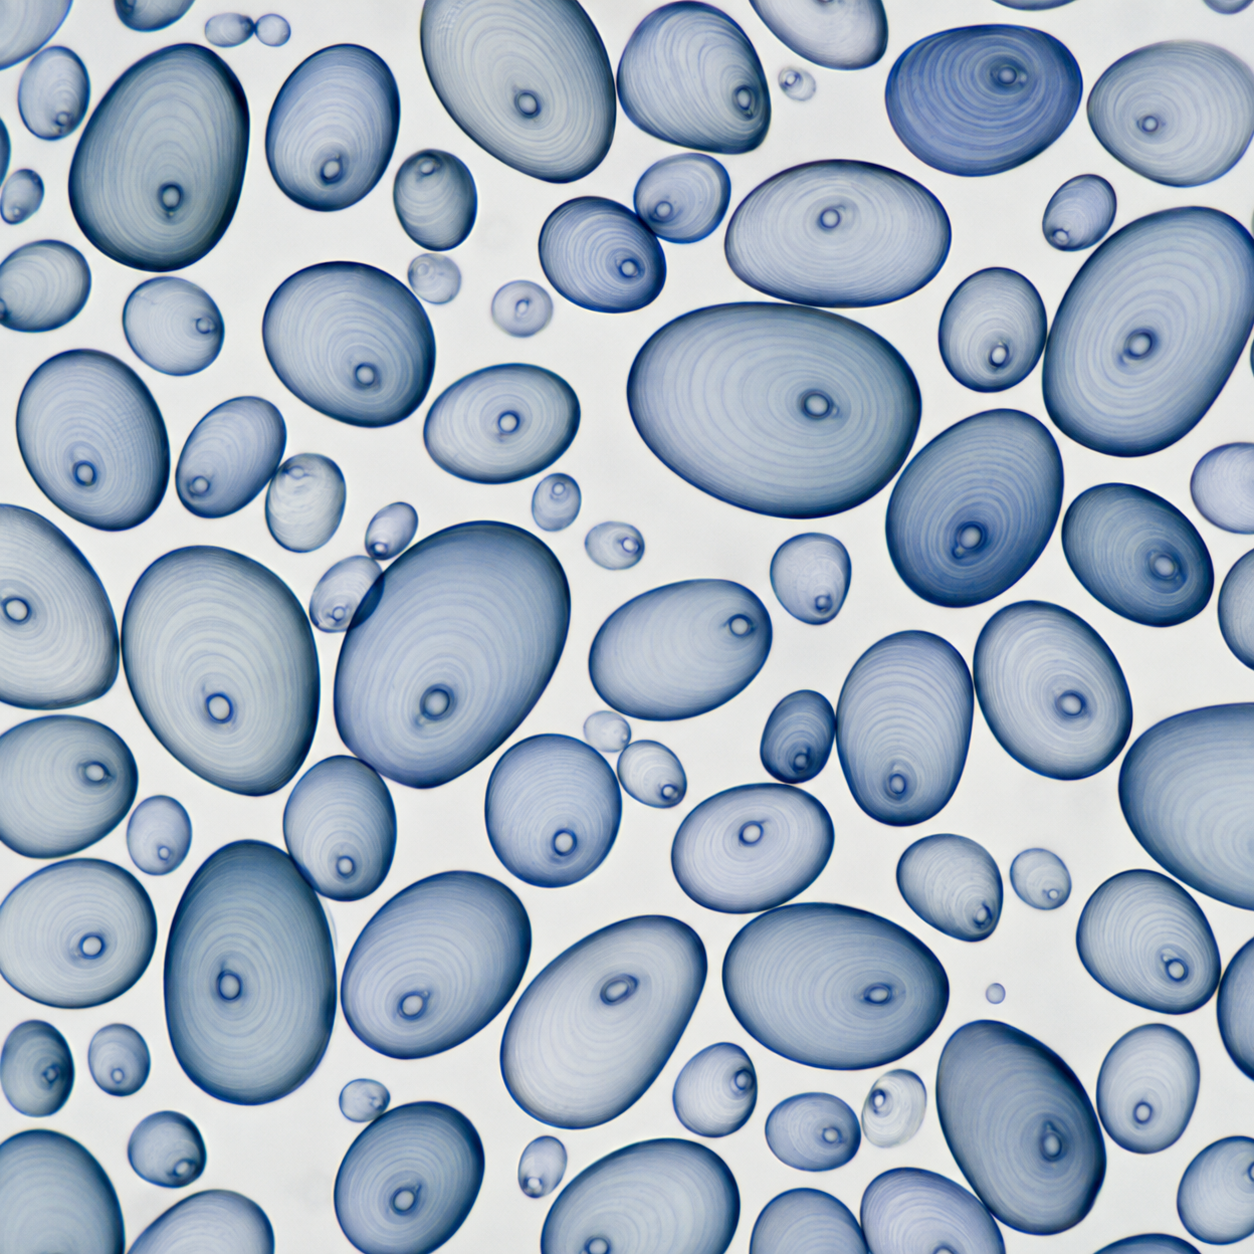
\includegraphics[width=0.96\linewidth]{images/book3/ai/b3-10-starch-grains.png}
\end{minipage}\hfill
\begin{minipage}[b]{0.52\linewidth}\centering
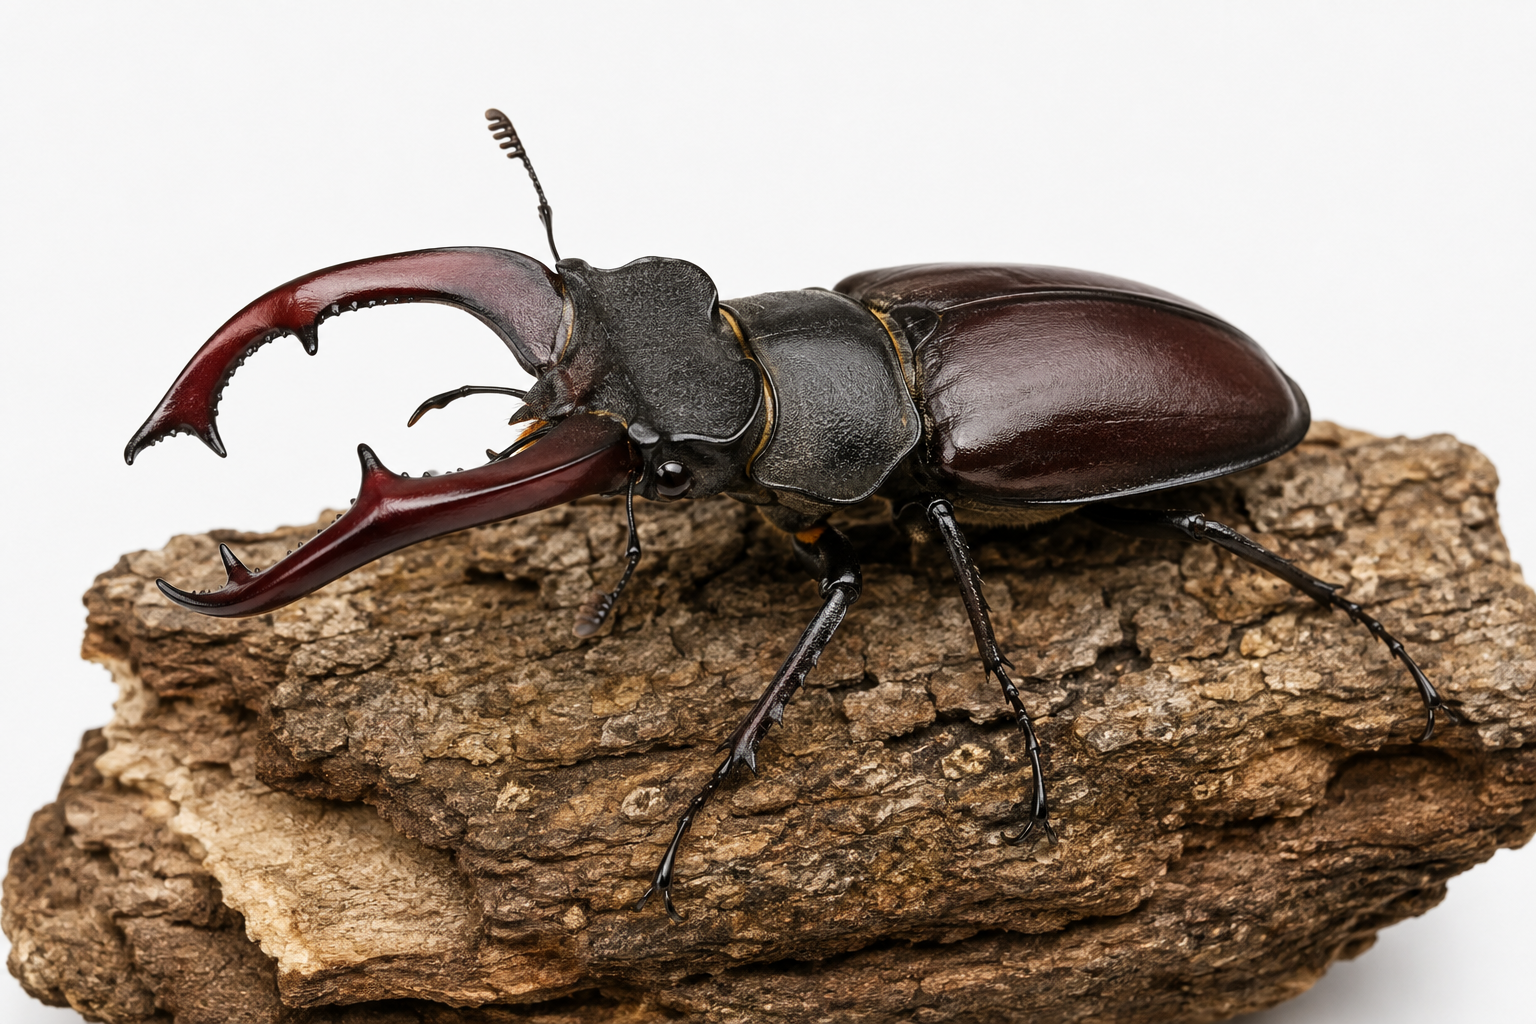
\includegraphics[width=0.96\linewidth]{images/book3/ai/b3-10-beetle-cuticle.png}
\end{minipage}

{\small बाएँ: सूक्ष्मदर्शी के नीचे आलू के मंड-कण, आयोडीन से रंगे; ये
संकेंद्री वलय ऐमाइलोपेक्टिन की उन परतों के हैं जो दिन-ब-दिन बिछाई गईं।
दाएँ: किसी सींगदार भृंग की \omterm{def:b1:flowering-plant-organization:tissues}{उपचर्म} --- किसी प्रोटीन आधात्री में \omterm{def:b1:carbohydrates:polysaccharide}{काइटिन}
तंतु, कड़े और गहरे: वही $\beta(1{\to}4)$ अभिकल्पना जो \omterm{def:b1:carbohydrates:polysaccharide}{सेलुलोस} की है, पर
एक अलग शर्करा पर।}
\end{omfigure}

\begin{example}[ग्लाइकोजन शाखित क्यों है]\label{ex:b1:carbohydrates:branching}
\omterm{def:b1:carbohydrates:polysaccharide}{ग्लाइकोजन} अपने अनपचायक सिरों से, एक बार में एक ग्लूकोज़, \omterm{def:b1:carbohydrates:polysaccharide}{ग्लाइकोजन}
फ़ॉस्फ़ोरिलेज़ द्वारा तोड़ा जाता है। \num{50000} ग्लूकोज़ की किसी
अशाखित शृंखला का ऐसा एक ही सिरा होता और वह प्रति एंजाइम-चक्र एक ग्लूकोज़
छोड़ती; और उतने ही आकार का कोई \omterm{def:b1:carbohydrates:polysaccharide}{ग्लाइकोजन} कण, जो हर बारह अवशेषों पर शाखित
है, कोई \num{2000} सिरे रखता है और एक साथ दो हज़ार छोड़ता है। शाखन कण को
संहत और घुलनशील भी बनाए रखता है। यकृत का सौ ग्राम \omterm{def:b1:carbohydrates:polysaccharide}{ग्लाइकोजन} दस ग्राम
प्रति घंटा की दर से जुटाया जा सकता है; वही ग्लूकोज़ एक लंबी शृंखला के
रूप में संचित होता तो खुलने में वर्षों लगते।
\end{example}

\begin{example}[ग्लूकोज़ को ही क्यों न संचित करें]\label{ex:b1:carbohydrates:osmotic}
सौ ग्राम ग्लूकोज़ (\qty{0.55}{mol}) किसी यकृत की \omterm{def:b1:cell-unit-of-life:cell}{कोशिकाओं} के
\qty{1}{L} जल में घुलकर \qty{0.3}{osmol/L} के किसी \omterm{def:b1:eukaryotic-cell:organelle}{कोशिकाद्रव} में
\qty{0.55}{osmol/L} और जोड़ देता: \omterm{def:b1:cell-unit-of-life:cell}{कोशिकाएँ} फूलकर अपने आयतन की तीन गुना
हो जातीं और फट जातीं। \omterm{def:b1:carbohydrates:polysaccharide}{ग्लाइकोजन} के रूप में वही ग्लूकोज़
$\num{7e18}$ कण हैं, यानी \qty{1e-5}{mol/L}, जो \omterm{def:b1:membranes-transport:osmosis}{परासरणी} दृष्टि से
अदृश्य है। कोई बहुलक अनेकानेक अणुओं को एक ही अणु के रूप में संचित करने का
ढंग है।
\end{example}

\section{ग्लाइकोसंयुग्म और पादप भित्ति}

\begin{definition}[ग्लाइकोप्रोटीन, प्रोटिओग्लाइकैन, ग्लाइकोलिपिड]\label{def:b1:carbohydrates:glycoconjugate}
शर्कराएँ प्रोटीनों और \omterm{def:b1:lipids:fattyacid}{लिपिडों} से सहसंयोजी रूप से जुड़कर
\emph{ग्लाइकोसंयुग्म}\index{ग्लाइकोसंयुग्म} बनाती हैं। कोई \emph{ग्लाइकोप्रोटीन}\index{ग्लाइकोप्रोटीन}
अपने कुछ ऐस्पैरजीन, सेरीन या थ्रिओनीन अवशेषों पर छोटी शाखित शृंखलाएँ
(दर्जन भर शर्कराएँ) धारण करता है, जो ER और \omterm{def:b1:eukaryotic-cell:endomembrane}{गॉल्जी} में जोड़ी जाती हैं
(\cref{ch:b1:eukaryotic-cell}): लगभग हर स्रावी और \omterm{def:b1:membranes-transport:membrane}{झिल्ली प्रोटीन} ऐसा ही
है। कोई \emph{प्रोटिओग्लाइकैन}\index{प्रोटिओग्लाइकैन} एक प्रोटीन
अंतर्भाग है जो दोहराती अम्लीय द्विशर्कराओं की लंबी अशाखित शृंखलाएँ
धारण करता है, यानी \emph{ग्लाइकोसैमीनोग्लाइकैन}\index{ग्लाइकोसैमीनोग्लाइकैन} (हायलूरोनन,
कॉन्ड्रॉइटिन सल्फ़ेट, हेपैरिन), जो बहुत बड़ी मात्रा में जल बाँधते हैं और
उपास्थि, काचाभ काय तथा \omterm{def:b1:body-plans-tissues:connective}{बाह्यकोशिकीय आधात्री} को उनकी प्रत्यास्थता देते
हैं। \emph{ग्लाइकोलिपिड}\index{ग्लाइकोलिपिड} प्लाज़्मा झिल्ली के बाहरी
पर्ण में किसी \omterm{def:b1:lipids:fattyacid}{लिपिड} पुच्छ पर शर्कराएँ धारण करते हैं। ग्लाइकोप्रोटीनों की
शर्कराओं के साथ मिलकर वे \emph{ग्लाइकोकैलिक्स}\index{ग्लाइकोकैलिक्स}
बनाते हैं, यानी वह शर्करा-आवरण जिससे \omterm{def:b1:cell-unit-of-life:cell}{कोशिकाएँ} पहचानी जाती हैं।
\end{definition}

\begin{example}[रक्त समूह]\label{ex:b1:carbohydrates:abo}
ABO रक्त समूह लाल \omterm{def:b1:cell-unit-of-life:cell}{कोशिका} की सतह के ग्लाइकोलिपिडों और
\omterm{def:b1:carbohydrates:glycoconjugate}{ग्लाइकोप्रोटीनों} पर की एक ही शर्करा-शृंखला के तीन रूप हैं: O शृंखला
फ़्यूकोस पर समाप्त होती है; A उसमें एक N-ऐसीटिलगैलैक्टोसामीन जोड़ता है,
B एक गैलैक्टोस, और यह एक ही एंजाइम के दो रूप करते हैं; और AB \omterm{def:b1:cell-unit-of-life:cell}{कोशिकाएँ}
दोनों धारण करती हैं। प्रतिरक्षा तंत्र को अपने और पराए में भेद करने के लिए,
और किसी आधान के सफल होने या मार डालने के लिए, एक ही शर्करा-अवशेष काफ़ी
है।
\end{example}

\begin{proposition}[पादप कोशिका भित्ति]\label{prop:b1:carbohydrates:wall}
\index{कोशिका भित्ति}
किसी पादप \omterm{def:b1:cell-unit-of-life:cell}{कोशिका} की प्राथमिक भित्ति एक तंतु-प्रबलित मिश्रित रचना है:
परतों में बिछे \omterm{def:b1:carbohydrates:polysaccharide}{सेलुलोस} सूक्ष्मतंतुक (द्रव्यमान का एक-चौथाई, तन्य
सामर्थ्य), जिन्हें \emph{हेमिसेलुलोस} आपस में बाँधते हैं (यानी वे शाखित
\omterm{def:b1:carbohydrates:polysaccharide}{बहुशर्कराएँ} जो सूक्ष्मतंतुकों से \omterm{def:b1:water-small-molecules:water}{हाइड्रोजन बंध} बनाती हैं और उनके बीच पुल
डालती हैं) और जो \emph{पेक्टिन} के किसी जेल में धँसे रहते हैं (यानी वे
अम्लीय \omterm{def:b1:carbohydrates:polysaccharide}{बहुशर्कराएँ} जो जल तथा कैल्सियम थामती हैं और मध्य पटलिका में
\omterm{def:b1:cell-unit-of-life:cell}{कोशिकाओं} को आपस में जोड़ती हैं), और कुछ प्रतिशत प्रोटीन। वह पतली होती है
(\qtyrange{0.1}{1}{\micro m}), जल तथा छोटे विलेयों के लिए पारगम्य, और
\qty{1}{MPa} \omterm{def:b1:eukaryotic-cell:plantcell}{स्फीति} थामने भर मज़बूत। जो \omterm{def:b1:cell-unit-of-life:cell}{कोशिकाएँ} बढ़ना बंद कर देती हैं वे
अधिक \omterm{def:b1:carbohydrates:polysaccharide}{सेलुलोस} और \emph{लिग्निन} वाली एक मोटी \emph{द्वितीयक भित्ति} जोड़
सकती हैं, यानी वह ऐरोमैटिक बहुलक जो उसे जलरोधी और कड़ा बनाता है: लकड़ी
द्वितीयक भित्तियाँ ही है।
\end{proposition}

\begin{omfigure}
\begin{tikzpicture}[font=\footnotesize, line cap=round]
  % matrix background
  \fill[omExo!8] (0,0) rectangle (8.4,3.6);
  % microfibrils: two layers of thick lines at different angles
  \foreach \y in {0.5,1.5,2.5,3.5} { \draw[line width=5pt, omDef!60] (0.2,\y-0.3) -- (8.2,\y-0.1); }
  \foreach \x in {1.2,3.2,5.2,7.2} { \draw[line width=5pt, omDef!35] (\x,0.1) -- (\x+0.6,3.5); }
  % hemicellulose tethers
  \foreach \x in {0.8,2.4,4.0,5.6,7.4} { \draw[thick, omProp] (\x,0.25) .. controls (\x+0.3,0.7) .. (\x+0.1,1.2) .. controls (\x-0.2,1.7) .. (\x+0.2,2.25) .. controls (\x+0.4,2.8) .. (\x,3.3); }
  % pectin gel dots
  \foreach \p in {(0.5,0.9),(1.9,2.9),(2.9,0.8),(4.6,2.1),(6.1,1.0),(6.9,3.1),(3.7,3.2),(7.9,1.9)} { \fill[omExo!70] \p circle (0.07); }
  % labels outside
  \node[anchor=west, align=left] at (8.7,3.0) {\textcolor{omDef!70!black}{सेलुलोस सूक्ष्मतंतुक}\\ (तन्य सामर्थ्य, परतों में)};
  \node[anchor=west, align=left] at (8.7,1.8) {\textcolor{omProp!80!black}{हेमिसेलुलोस}\\ (तंतुकों को बाँधते हैं)};
  \node[anchor=west, align=left] at (8.7,0.6) {\textcolor{omExo!70!black}{पेक्टिन जेल}\\ (जलयोजित आधात्री, सीमेंट)};
\end{tikzpicture}

{\small एक मिश्रित रचना के रूप में प्राथमिक पादप \omterm{prop:b1:carbohydrates:wall}{कोशिका भित्ति}: पेक्टिन
के किसी जेल (हरा) में \omterm{def:b1:carbohydrates:polysaccharide}{सेलुलोस} सूक्ष्मतंतुकों (नीला) की परतें, जिन्हें
हेमिसेलुलोस शृंखलाएँ (नारंगी) बाँधती हैं। गीली आधात्री में कड़े तंतु:
काँच-तंतु की वही अभिकल्पना, जो एक अरब वर्ष पहले खोज ली गई थी।}
\end{omfigure}

\section{ईंधन और कार्बन के रूप में शर्कराएँ}

\begin{proposition}[ग्लूकोज़ का स्थान]\label{prop:b1:carbohydrates:fuel}
\omterm{def:b1:carbohydrates:monosaccharide}{कार्बोहाइड्रेट} ऑक्सीकरण पर \qty{17}{kJ/g} देते हैं और वह ईंधन हैं जिसे
हर \omterm{def:b1:cell-unit-of-life:cell}{कोशिका} काम में ले सकती है, ऑक्सीजन के साथ या उसके बिना
(\cref{ch:b1:respiration-fermentation});
ग्लूकोज़ रक्त की शर्करा है (\qty{5}{mmol/L}), सुक्रोस पादप रस की, और
\omterm{def:b1:carbohydrates:polysaccharide}{मंड} तथा \omterm{def:b1:carbohydrates:polysaccharide}{ग्लाइकोजन} उनके भंडार। शर्कराएँ वह कार्बन भी हैं जिनसे \omterm{def:b1:cell-unit-of-life:cell}{कोशिका}
बाक़ी सब कुछ बनाती है: न्यूक्लियोटाइडों के पेंटोस, \omterm{def:b1:lipids:fattyacid}{लिपिडों} का ग्लिसरॉल,
ऐमीनो अम्लों के कार्बन कंकाल --- सब शर्करा-पथों से निकलते हैं
(\cref{ch:b1:biosyntheses-integration})।
प्रकाश-संश्लेषण पहले शर्करा बनाता है; बाक़ी सब उसके पीछे आता है।
\end{proposition}

\begin{example}[एक दिन की शर्करा]\label{ex:b1:carbohydrates:day}
मनुष्य दिन में कोई \qty{300}{g} \omterm{def:b1:carbohydrates:monosaccharide}{कार्बोहाइड्रेट} खाता है, लगभग सारा \omterm{def:b1:carbohydrates:polysaccharide}{मंड}
और सुक्रोस के रूप में; आँत उसका \omterm{prop:b1:water-small-molecules:families}{जल-अपघटन} करके ग्लूकोज़, फ्रक्टोस और
गैलैक्टोस बनाती है, यकृत बाद के दोनों को ग्लूकोज़ में बदल देता है, और
ग्लूकोज़ पूरे रक्त में \qty{5}{g} पर घूमता रहता है --- यानी मस्तिष्क के
लिए बीस मिनट की आपूर्ति, जो दिन में \qty{120}{g} लेता है, और जो यकृत के
\omterm{def:b1:carbohydrates:polysaccharide}{ग्लाइकोजन} से लगातार भरी जाती रहती है। आँख का लेंस, लाल \omterm{def:b1:cell-unit-of-life:cell}{कोशिकाएँ} और गुर्दे
की मध्यांश केवल ग्लूकोज़ पर जीते हैं; आहार में और कुछ उसकी जगह नहीं ले
सकता, और वह चुक जाने पर यकृत उसे प्रोटीन से बनाता है।
\end{example}

\section{अभ्यास}

\begin{exercise}[$\star$]\label{exo:b1:carbohydrates:1}
ग्लूकोज़, फ्रक्टोस, राइबोस और ग्लिसरैल्डिहाइड को कार्बनों की संख्या से
और \omterm{def:b1:carbohydrates:monosaccharide}{ऐल्डोस} या \omterm{def:b1:carbohydrates:monosaccharide}{कीटोस} होने से वर्गीकृत कीजिए।
\end{exercise}

\begin{exercise}[$\star$]\label{exo:b1:carbohydrates:2}
ऐनोमरी कार्बन क्या है, और जिस \omterm{def:b1:carbohydrates:glycosidic}{द्विशर्करा} के दोनों ऐनोमरी कार्बन बंध में
हों वह बेनेडिक्ट अभिकर्मक से क्रिया क्यों नहीं करती?
\end{exercise}

\begin{exercise}[$\star$]\label{exo:b1:carbohydrates:3}
\omterm{def:b1:carbohydrates:polysaccharide}{मंड}, \omterm{def:b1:carbohydrates:polysaccharide}{ग्लाइकोजन}, \omterm{def:b1:carbohydrates:polysaccharide}{सेलुलोस} और \omterm{def:b1:carbohydrates:polysaccharide}{काइटिन} के एकलक और बंध बताइए।
\end{exercise}

\begin{exercise}[$\star$]\label{exo:b1:carbohydrates:4}
हावर्थ वाले आलेख से $\alpha$-D-ग्लूकोज़ के कार्बन 1 से 4 तक के
हाइड्रॉक्सिलों की स्थितियाँ (ऊपर या नीचे) गिनाइए, फिर
$\alpha$-D-गैलैक्टोस बनाइए या उसका वर्णन कीजिए।
\end{exercise}

\begin{exercise}[$\star\star$]\label{exo:b1:carbohydrates:5}
$\alpha$ और $\beta$ बंधों की ज्यामिति से समझाइए कि ऐमाइलोस कुंडली और
\omterm{def:b1:carbohydrates:polysaccharide}{सेलुलोस} फ़ीता क्यों बनाता है, और आयोडीन की जाँच पहले पर क्यों काम करती है
और दूसरे पर नहीं।
\end{exercise}

\begin{exercise}[$\star\star$]\label{exo:b1:carbohydrates:6}
तीन नलियों में ग्लूकोज़, सुक्रोस और \omterm{def:b1:carbohydrates:polysaccharide}{मंड} हैं। जाँचों का ऐसा क्रम
(बेनेडिक्ट, आयोडीन, अम्लीय \omterm{prop:b1:water-small-molecules:families}{जल-अपघटन}) रचिए जो हर एक की पहचान कर दे, और हर
जाँच का अपेक्षित परिणाम दीजिए।
\end{exercise}

\begin{exercise}[$\star\star$]\label{exo:b1:carbohydrates:7}
किसी \omterm{def:b1:carbohydrates:polysaccharide}{ग्लाइकोजन} कण में \num{50000} ग्लूकोज़ अवशेष हैं और वह हर 12 पर
शाखित है। अनपचायक सिरों की संख्या आँकिए और उतने ही आकार के किसी ऐमाइलोस
अणु से तुलना कीजिए। यदि फ़ॉस्फ़ोरिलेज़ हर सिरे से प्रति सेकंड एक
ग्लूकोज़ छोड़े, तो हर एक को अपने ग्लूकोज़ का \qty{10}{\%} छोड़ने में
कितना समय लगेगा?
\end{exercise}

\begin{exercise}[$\star\star$]\label{exo:b1:carbohydrates:8}
\omterm{def:b1:carbohydrates:polysaccharide}{सेलुलोस} सूक्ष्मतंतुकों की तन्य सामर्थ्य लगभग \qty{1}{GPa} है।
\qty{50}{\micro m} व्यास और \qty{0.5}{\micro m} मोटी भित्ति वाली कोई
\omterm{def:b1:cell-unit-of-life:cell}{कोशिका} \qty{0.8}{MPa} \omterm{def:b1:eukaryotic-cell:plantcell}{स्फीति} थामती है। भित्ति में प्रतिबल निकालिए
(किसी गोले के लिए $\sigma = Pr/2t$) और सामर्थ्य से तुलना कीजिए।
\end{exercise}

\begin{exercise}[$\star\star$]\label{exo:b1:carbohydrates:9}
लैक्टोस असहिष्णुता: जिन वयस्कों में आँत की लैक्टेज़ नहीं होती उन्हें दूध
के बाद मरोड़ और अतिसार होते हैं। लैक्टेज़ जिस बंध को तोड़ती है उससे
समझाइए कि बिना पचे लैक्टोस का बृहदांत्र में क्या होता है (जीवाणु,
\omterm{def:b1:membranes-transport:osmosis}{परासरण})।
\end{exercise}

\begin{exercise}[$\star\star\star$]\label{exo:b1:carbohydrates:10}
कोई गाय दिन में \qty{10}{kg} घास का शुष्क पदार्थ खाती है, जिसका
\qty{40}{\%} \omterm{def:b1:carbohydrates:polysaccharide}{सेलुलोस} है। उसके पास कोई सेलुलेज़ नहीं है। समझाइए कि फिर भी
वह \omterm{def:b1:carbohydrates:polysaccharide}{सेलुलोस} से ऊर्जा कैसे पाती है, यह प्रक्रिया छोटी आँत से पहले क्यों
होनी चाहिए, और यदि \qty{60}{\%} \omterm{def:b1:carbohydrates:polysaccharide}{सेलुलोस} किण्वित हो और प्रति ग्राम
\qty{12}{kJ} उपयोगी उत्पाद दे तो दाँव पर लगी ऊर्जा आँकिए।
\end{exercise}

\begin{exercise}[$\star\star\star$]\label{exo:b1:carbohydrates:11}
A और B रक्त-समूह प्रतिजन एक शर्करा से भिन्न हैं जिसे किसी
हस्तांतरेज़ के दो रूप जोड़ते हैं; O प्ररूप में कोई नहीं होता। समझाइए कि
कोई O व्यक्ति अपनी लाल \omterm{def:b1:cell-unit-of-life:cell}{कोशिकाएँ} किसी को भी क्यों दे सकता है पर केवल O से
ही क्यों ले सकता है, और किसी A व्यक्ति के प्लाज़्मा में क्या होना चाहिए।
\end{exercise}

\begin{exercise}[$\star\star\star$]\label{exo:b1:carbohydrates:12}
``ग्लूकोज़ सार्वत्रिक ईंधन है, \omterm{def:b1:carbohydrates:polysaccharide}{सेलुलोस} सार्वत्रिक निर्माण-सामग्री, और वे
एक ही अणु हैं।'' एक अनुच्छेद में चर्चा कीजिए: यह वाक्य क्या ठीक कहता है,
एक बंध क्या बदल देता है, और यह रसायन तथा जीवविज्ञान के संबंध के बारे में
क्या कहता है।
\end{exercise}

\section{समस्या: ग्लाइकोजन का वृक्ष}

\begin{problem}[{सप्ताहांत समस्या --- शाखा-दर-शाखा गिना गया एक
ग्लाइकोजन कण, तौला गया और समयबद्ध किया गया यकृत का भंडार, वह परासरणी
क़ीमत जिससे बहुलकीकरण बचाता है, और अंत में यकृत की ग्लूकोज़-निर्मुक्ति
दर}]
\label{pb:b1:carbohydrates:1}
कोई \omterm{def:b1:carbohydrates:polysaccharide}{ग्लाइकोजन} कण शृंखलाओं का एक वृक्ष है: \qty{13}{} ग्लूकोज़ अवशेषों की
एक भीतरी शृंखला दो शाखाएँ धारण करती है, जिनमें से हर एक \qty{13}{}
अवशेषों की है और हर एक बदले में दो शाखाएँ धारण करती है, और यही
\qty{12}{} स्तरों तक चलता है; और सबसे बाहरी स्तर की शृंखलाएँ अशाखित हैं।
बहुलक में हर ग्लूकोज़ अवशेष का द्रव्यमान \qty{162}{g/mol} है। विश्राम कर
रहे किसी मनुष्य के \qty{1.5}{kg} यकृत में \qty{1.0}{L} कोशिका-जल में
\qty{100}{g} \omterm{def:b1:carbohydrates:polysaccharide}{ग्लाइकोजन} है, और वह भोजनों के बीच रक्त में
\qty{10}{g/h} की दर से ग्लूकोज़ छोड़ता है। \omterm{def:b1:carbohydrates:polysaccharide}{ग्लाइकोजन} फ़ॉस्फ़ोरिलेज़
प्रति चक्र किसी अनपचायक सिरे से एक ग्लूकोज़ हटाती है, और प्रति एंजाइम अणु
प्रति सेकंड \qty{20}{} चक्र लगाती है।

\medskip
\noindent\textbf{भाग I --- वृक्ष की गिनती।}
\begin{enumerate}
  \item स्तर $t$ में कितनी शृंखलाएँ हैं (भीतरी शृंखला के लिए
        $t = 1$)? स्तर 1, 2, 3 और 12 के लिए संख्या दीजिए।
  \item कण में शृंखलाओं की कुल संख्या निकालिए।
  \item ग्लूकोज़ अवशेषों की कुल संख्या निकालिए।
  \item कण का द्रव्यमान डाल्टन में और ग्राम में निकालिए।
  \item सारी शृंखलाओं का कितना भिन्न सबसे बाहरी स्तर में है? कण कितने
        अनपचायक सिरे देता है?
  \item उतने ही अवशेषों के किसी ऐमाइलोस अणु के कितने अनपचायक सिरे
        होंगे?
  \item यदि हर स्तर त्रिज्या में \qty{1.9}{nm} जोड़े, तो कण का व्यास
        निकालिए और उसकी तुलना किसी राइबोसोम
        (\qty{25}{nm}) से कीजिए।
\end{enumerate}

\medskip
\noindent\textbf{भाग II --- यकृत का भंडार।}
\begin{enumerate}[resume]
  \item यकृत में कणों की संख्या निकालिए।
  \item यह भंडार जितना ग्लूकोज़ है वह मोल में और मुक्त ग्लूकोज़ के
        ग्राम में निकालिए (\qty{180}{g/mol})।
  \item \omterm{def:b1:carbohydrates:polysaccharide}{ग्लाइकोजन} प्रति ग्राम \qty{3}{g} जल बाँधता है। यकृत का कितना
        द्रव्यमान \omterm{def:b1:carbohydrates:polysaccharide}{ग्लाइकोजन} और उसका जल है?
  \item \qty{10}{g/h} की निर्मुक्ति दर को प्रति सेकंड ग्लूकोज़ अणुओं
        में निकालिए।
  \item उस दर पर भंडार कितने घंटे चलता है? यह निर्मुक्ति मुख्यतः किस \omterm{def:b1:mammal-organization:organ}{अंग}
        की माँग पूरी करती है?
\end{enumerate}

\medskip
\noindent\textbf{भाग III --- सिरे और एंजाइम।}
\begin{enumerate}[resume]
  \item यकृत में अनपचायक सिरों की कुल संख्या निकालिए।
  \item यदि हर सिरे पर एक साथ प्रति सेकंड \qty{20}{} ग्लूकोज़ की दर से
        हमला हो, तो निर्मुक्ति दर ग्राम प्रति सेकंड में क्या होती?
        असली दर से तुलना कीजिए।
  \item असली दर के लिए कितने फ़ॉस्फ़ोरिलेज़ अणु चाहिए, यदि हर एक प्रति
        सेकंड \qty{20}{} की दर से काम करे?
  \item मान लीजिए वही \qty{100}{g} कणों जितने ही आकार की ऐमाइलोस
        शृंखलाओं के रूप में संचित हों। सिरों की संख्या और अधिकतम
        निर्मुक्ति दर निकालिए।
  \item समझाइए कि रक्त-ग्लूकोज़ के गिरने पर यकृत की मिनटों के भीतर की
        अनुक्रिया की कुंजी शाखा-बिंदु ही क्यों हैं।
\end{enumerate}

\medskip
\noindent\textbf{भाग IV --- \omterm{def:b1:membranes-transport:osmosis}{परासरणी} क़ीमत।}
\begin{enumerate}[resume]
  \item यदि वे \qty{100}{g} \qty{1.0}{L} कोशिका-जल में मुक्त ग्लूकोज़
        के रूप में घुले हों, तो वे कितनी परासरणीयता जोड़ते?
  \item \omterm{def:b1:eukaryotic-cell:organelle}{कोशिकाद्रव} की \qty{0.3}{osmol/L} से तुलना कीजिए और भविष्यवाणी
        कीजिए कि \omterm{def:b1:cell-unit-of-life:cell}{कोशिकाओं} का क्या होता।
  \item स्वयं \omterm{def:b1:carbohydrates:polysaccharide}{ग्लाइकोजन} कणों से मिली परासरणीयता निकालिए।
  \item मुक्त ग्लूकोज़ जो \omterm{def:b1:membranes-transport:osmosis}{जल विभव} बनाता वह निकालिए
        ($\Psi_s = -RTc$, $RT = \qty{2.58}{MPa.L/mol}$) और वह दाब भी जो
        किसी पादप जैसी भित्ति को उसका सामना करने के लिए चाहिए होता।
  \item पेशी \qty{30}{kg} पेशी में \qty{400}{g} \omterm{def:b1:carbohydrates:polysaccharide}{ग्लाइकोजन} संचित करती है
        पर रक्त में ग्लूकोज़ नहीं छोड़ सकती। पेशी में \omterm{def:b1:carbohydrates:polysaccharide}{ग्लाइकोजन} जिस काम
        के लिए है उसे देखते हुए इसका कारण सुझाइए।
  \item कोई आलू \omterm{def:b1:carbohydrates:polysaccharide}{मंड} को \qty{50}{\micro m} के कणों में संचित करता है,
        \qty{40}{nm} के \omterm{def:b1:carbohydrates:polysaccharide}{ग्लाइकोजन} कणों में नहीं। इस भेद को हर \omterm{def:b1:organism-environment:organism}{जीव} को
        चाहिए जुटाव-कालमान से जोड़िए।
  \item भोजन के बाद यकृत चार घंटे में \qty{100}{g} \omterm{def:b1:carbohydrates:polysaccharide}{ग्लाइकोजन} फिर बना
        लेता है। दर को प्रति सेकंड ग्लूकोज़ अवशेषों में निकालिए और यदि
        एक अवशेष जोड़ने में दो \omterm{def:b1:water-small-molecules:atp}{ATP} तुल्यांक लगते हों तो \omterm{def:b1:water-small-molecules:atp}{ATP} की लागत भी।
  \item परिणाम बताइए: यकृत की ग्लूकोज़-निर्मुक्ति दर प्रति सेकंड अणुओं
        में, वे अनपचायक सिरे जो उसे संभव बनाते हैं, और वह परासरणीयता जो
        बहुलक \omterm{def:b1:cell-unit-of-life:cell}{कोशिकाओं} को बचा देता है।
\end{enumerate}
\end{problem}
